% Optional Introduction
\chapter{Introduction}

Computer security is an inherently adversarial discipline in which
each ``side'' seeks to exploit the assumptions and limitations of the
other.  Attackers rely on exploiting knowledge of vulnerabilities,
configuration errors or operational lapses in order to penetrate
targeted systems, while defenders in turn seek to improve their
resistance to such attacks by better understanding the nature of
contemporary threats and the technical fingerprints left by attacker's
craft.  Invariably, this means that attackers are driven to innovate
and diversify while defenders, in response, must continually monitor
for such changes and update their operational security practices
accordingly.  This dynamic is present in virtually every aspect of the
operational security landscape, from anti-virus signatures to the
configuration of firewalls and intrusion detection systems to incident
response and triage.  Common to all such reifications, however, is the
process of monitoring for new data on attacker behavior and using that
data to update defenses and security practices. Indeed, the extent to
which a defender is able to gather and analyze such data effectively
defines a de facto window of vulnerability---the time during which an
organization is less effective in addressing attacks due to ignorance
of current attacker behaviors.

This abstract problem has given rise to a concrete demand for
contemporary threat data sources that are frequently collectively
referred to as \emph{threat intelligence}. Threat Intelligence 
is the \emph{knowledge} that allows organizations to understand and 
mitigate cyber-attacks. This ``knowledge'' involves a wide variety 
of things. It can be vulnerability reports, where system and 
network administrators can learn the vulnerabilities and the potential
impact on their systems. It can also be IP or domain blacklists,
which tell users where the attacks are originating from, so people
can take precautions against these indicators. It can even be some 
online discussion thread in an underground forum, so security 
experts can track what malicious actors are discussing about. 
All of these knowledge can help security experts better understand 
potential threats, and then better help organizations to defend 
against them.

By far the most common form of Threat Intelligence are so-called 
\emph{indicators of compromise:} simple observable behaviors that 
signal that a host or network may be compromised. These indicators 
are in general straightforward forensic data that are directly 
associated with attacks. The most notable examples are:
\begin{prettylist}
    \item \textbf{IP Addresses}: IPs known to launch particular 
    attacks, like port scanning, brute-force login, etc.
    \item \textbf{Domain Addresses}: Domains known to host 
    Command-and-Control servers or sending spam emails, etc.
    \item \textbf{URLs}: Compromised websites or phish URLs, etc.
    \item \textbf{File Hashes}: Indicating a file or executable 
    known to be associated with a particular variety of malware, etc.
\end{prettylist}

The presence of such indicators in a system or network is a symptom 
that alerts an organization to a problem. For example, if one 
machine in an organization contacted a domain that known to be
associated with malware Command-and-Control servers, it is a strong
indication that this machine is probably infected with the 
corresponding malware. Part of an organization's defenses 
should reasonably include monitoring its assets
for such indicators to detect and mitigate potential compromises as
they occur. And these indicators are simple enough that they can be
easily integrated into defense or monitoring systems, like network
firewalls or malware scanners.

While each organization naturally collects a certain amount of threat
intelligence data on its own (e.g., the attacks they repel, the e-mail
spam they filter, etc.). any single entity has a limited footprint and
few are instrumented to carefully segregate crisp signals of attacks
from the range of ambiguity found in normal production network and
system logs. Thus, it is now commonly accepted that threat
intelligence data procurement is a specialized activity whereby
third-party firms, and/or collections of public groups, employ a range
of monitoring techniques to aggregate, filter and curate quality
information about current threats.  Indeed, the promised operational
value of threat intelligence has created a thriving (multi-billion
dollar) market~\cite{timarket}. 

Most established security firms, like Cisco Security~\cite{ciscotalos}, 
Palo Alto Networks~\cite{panautofocus}, Fortinet~\cite{fortinet} etc, 
and many specialized companies, like CrowdStrike~\cite{crowdstrike}, 
Anomali ThreatStream~\cite{anomali}, Recorded Future~\cite{recordedfuture}
etc,. are all offering threat intelligence solutions. Public threat
intelligence providers like Spamhaus, Abuse.ch, Dshield etc, are also 
getting more and more attentions. The global threat intelligence market is
predicated to surpass \$13 Billion in 2025~\cite{tipredict2018}. With the
industry thriving, there is also a rapid increase in the related research
works~\cite{tounsi2018survey}, covering topics from data characteristic,
effectiveness evaluation to design better sharing systems and protocols.

From a high level, there are two major aspects of Threat Intelligence: 
\textit{Data} and \textit{Operation}. \textit{Data} represents the content 
of Threat Intelligence---the actual information provided in different Threat
Intelligence products. \textit{Operation} represents the usage of 
data---different ways people can use Threat Intelligence to help. This
generalization is common for all data-based products. Therefore,
all research problems related to Threat Intelligence can be categorized into
these two areas: analyzing threat intelligence data itself, or exploring
ways to use the data.

When looking at these two general problems, one can further 
take two different research approaches: \textit{Empirical} and 
\textit{Algorithmic}. \textit{Empirical} approach focuses on understanding
the current ecosystem of Threat Intelligence, including studying the 
data characteristic, measuring different use cases, discover potential 
shortcomings, etc. This approach emphasizes on thoroughly understanding
existing solutions, uncovering patterns and underlying logic, 
so the community can gain valuable insights.
\textit{Algorithmic} approach, on the other hand, 
focuses on designing new algorithms to 
improve current solutions, like new threat hunting algorithms to improve 
Threat Intelligence data quality, or better ways to utilize these data 
during operation, etc. This approach emphasizes on designing new solutions 
to improve existing ones, so the community can have better algorithms and
tools to work with Threat Intelligence.

\begin{figure}
\centering
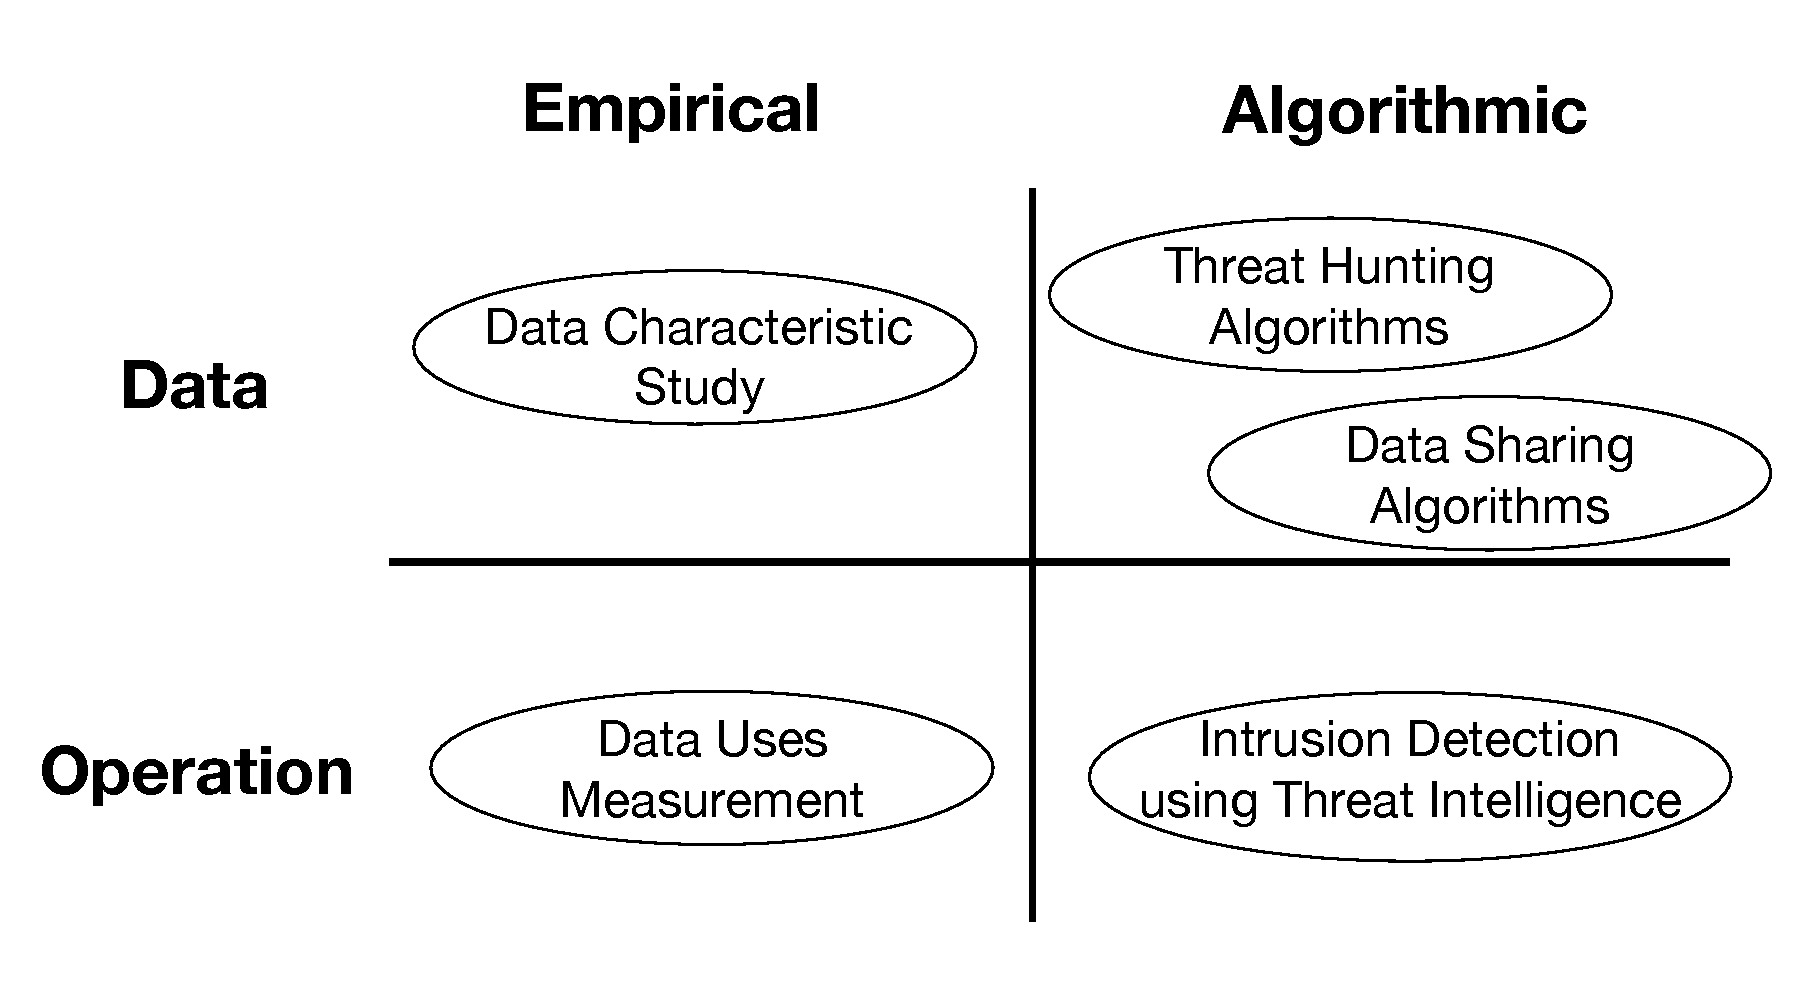
\includegraphics[width=0.8\textwidth]{threat_intel_research_overview.pdf}
\caption{Threat Intelligence research overview and example research
topics in each direction.}
\label{fig:threat_intel_overview}
\end{figure}

Therefore, research directions related to Threat Intelligence can be 
viewed in four general categories, as illustrated in
Figure~\ref{fig:threat_intel_overview}. More specifically, the four 
research directions are: 
\begin{prettylist}
    \item Empirical analysis on Threat Intelligence data: \\
    Understanding the characteristic of Threat Intelligence data, different
    data generation systems and their performance, different threat sharing
    strategies and how are they being used in the real-world, etc.
    
    \item Algorithm exploration related to Threat Intelligence data: \\
    Designing algorithms for threat hunting (Threat Intelligence generation),
    specification for data description and protocols for data sharing, etc.
    
    \item Empirical analysis on Threat Intelligence usage: \\
    Measuring how organizations are using Threat Intelligence, the problems 
    when using these data and the impact on the Internet, etc.
    
    \item Algorithm exploration related to Threat Intelligence usages: \\
    Designing better methods to use threat intelligence during system and 
    network defense(e.g. increasing coverage, reducing false positives),
    explore new ways to use threat intelligence data, such as using the 
    data as machine learning training data, etc.
\end{prettylist}

In this dissertation, I take an empirical approach and explore the 
\textit{Data} and \textit{Operation} problems of Threat Intelligence.
I focus on thoroughly understanding the current status of Threat 
Intelligence and will then discuss my takeaways from these analyses.
In the study of \textit{Data}, which will be discussed in Chapter~\ref{chapter:data_character}, 
I analyzed the data characteristics of existing Threat Intelligence products.
I designed mathematics metrics for Threat Intelligence data evaluation,
and with these metrics, I studied \numipfeeds\ distinct IP address 
data feeds, covering six categories of threats, and \numhashfeeds\ distinct
malware file hash feeds, and measured their data characteristic. Through this
work, I revealed the limitation of existing Threat Intelligence data and 
discussed the potential improvements based on my findings. In the study of
\textit{Operation}, which will be discussed in Chapter~\ref{chapter:data_usage},
I measured how Threat Intelligence data is being used on a large scale. 
I designed a method using IP ID side channel that can measure the 
connectivity between two Internet hosts from a third point. With this 
method, I conducted a large scale Internet measurement over {\reflroughnum} 
U.S. hosts and uncovered their uses of {\blacklistnum} popular public IP
blacklists. I further investigated a broader use of blacklists among the 
hosts, and discovered over 73K hosts has shown blacklist related blocking 
behavior. Together, my work provided an in-depth look into the current
status of Threat Intelligence and augmented the knowledge of our community
on this topic.

%\verb!\mainmatter! macro because it should start on page~1.
%\end{dissertationintroduction}
